\documentclass[10pt, onecolumn, draftclsnofoot, letterpaper,compsoc]{IEEEtran}
\usepackage[utf8]{inputenc}

\title{Capstone Requirements Document}
\author{GFR Group \\
            CS461 Senior Software Engineering Project \\
            Fall 2018 \\
            \today}

\usepackage{natbib}
\usepackage{graphicx}

\begin{document}

\maketitle
%\begin{abstract} SUBJECT TO CHANGE

Autonomous vehicles require robust representations of the world in order to make correct driving decisions. The driverless vehicle must utilize sensor input from lidar, camera, accelerometer and GPS in order to construct a virtual representation of the world around it as well as localize itself within that world. Due to the inherent error and low sampling rates of the sensors, high speed motion can cause data about the environment to be sparse and noisy. Robust statistical analysis is needed to evaluate the confidence of the vehicle's internal representation of the world around it. Our team is tasked with constructing the vision, mapping, and localization systems for a driverless formula style racecar for the Global Formula Racing (GFR) team. The driverless vehicle is expected to compete in the Formula SAE (FSAE) competition in August 2019. 

%\end{abstract}

\newpage
\tableofcontents
\newpage

\section{Introduction}

\subsection{Terminologies}

\begin{itemize}
    \item \textbf{Lidar} A visual sensor that fundamentally works like a radar but uses lasers instead of radio waves
    \item \textbf{GPS} Global Positioning System
    \item \textbf{IMU} Inertial Measurement Unit
    \item \textbf{ROS} Robot Operating System
    \item \textbf{SSD} Single Shot Multibox Detector
    \item \textbf{mAP} mean Average Percision
    \item \textbf{SIFT} Scale Invariant Feature Transform
    \item \textbf{SLAM} Simutaneously Localization And Mapping 
    \item \textbf{EKF} Extended Kalman Filter
    \item \textbf{GFR} Global Formula Racing
\end{itemize}

\subsection{Scope}

The purpose of our system is to create a robust virtual representation of the vehicle's environment. The virtual representation will be generated using sensor input from the camera, lidar, GPS, and IMU. Algorithms will be developed for detecting the location and color of the cones using lidar and camera. The cone locations and colors will be used to construct a dynamic map of the world, updating the map as the vehicle moves and new cones are seen. As the vehicle moves, our system will need to update the position of the vehicle within the map. The location of the vehicle and cones will be used to compute the optimal path and velocity to successfully maneuver around the track.

\section{Requirements}

\subsection{Vision}
\subsubsection{Camera}
The camera vision system should be able to accurately detect all cones within a sufficient distance from the camera. The vision system will be contained within a ROS node which takes in individual frames and output probabilities for x and y locations of all cones as well as the standard deviation of the cone's location in the x and y direction and the color of each cone. The node should also output the predicted distance of the cones in the x and y direction relative to the vehicle. Cones will be detected utilizing a combination of SSD and SIFT. SSD will be used to do the initial object detection and SIFT will then be used to track key points in the image through time in order to accurately find the centers of cones as well as estimates for the velocity of the vehicle. 

In order to utilize an SSD model, the model must be trained on a dataset of blue, yellow, and orange traffic cones. The dataset should contain a minimum of 40 ground truth images containing at least 100 blue and yellow cones and 30 orange cones. 40 images should should be sufficient enough to train a model to get relatively good classification and bounding box accuracies. Our goal is to achieve .75 mAP; e.g. 75\% of all predicted pixels should overlap their corresponding ground truth bounding boxes. We chose this accuracy goal as it is the highest mAP achieved on the original SSD paper. The SSD should also run at a minimum of 1 frame per foot of distance travelled in the vehicle. That is 88 frames per second when going 60 miles per hour. 

\subsubsection{Lidar}
Physically mounted on the chassis of the car, the lidar must continuously scan the 3 dimensional physical environment around the car as the car is moving at a speed of at most 60 miles per hour until being turned off, and also must continuously send the scanning data to the lidar processing component. 

These scanning data will be computationally processed by a lidar processing algorithm and then gives out the cone detection results and send this result to the Sensor Fusion component of the system. This lidar processing algorithm must be able to detect the relative 3D distances from the cones on both the left and the right boundaries ahead of the car to the location of the mounted lidar on the car.

\subsection{SLAM}
An important aspect of any autonomous vehicle is the ability to know its environment and where it exists in that environment. SLAM would allow the vehicle to both map out the environment without prior knowledge, and know the vehicle's location. The SLAM system will need to take inputs from lidar and camera ROS nodes. These outputs will include location of cones relative to the car, the color of the cone, and the standard deviation of the cone location. These cones will be used as landmarks for the track. No other landmarks will be used.

A crucial part of the SLAM criteria is knowing the environment in which the car is passing through. This includes knowing where the cones are located and using that data to ensure the car is in the desired location. Once the environment is known, the car needs to be aware of its location in that environment. This is when localization comes into play. Localization is the coordinates of the car in the layout created by the mapping section of SLAM. Since this is a competition, knowing the car's location will allow us to stay on track while optimizing our speed. Simulations will be run in Gazebo or rviz to validate the accuracy of our algorithm. 


% mention running in Gazebo/rviz simulations in order to validate quality of map

\subsection{Sensor Analysis}

To better localize the vehicle within its represented world, several orientation and location sensors are used on the vehicle. Three accelerometers and a GPS will provide some acceleration and position data, but double integrating a noisy accelerometer reading will lead to a position measurement that is unreliable at best, completely inaccurate at worst. To get usable odometry measurements, it will be necessary to filter the incoming sensor data. Because localization and mapping are heavily dependent on reliable odometry data, it is necessary to minimize uncertainty in measurements. 

The most basic requirement of proper sensor measurement is convergence and stability. The estimated vehicle state should approach the true vehicle state over time and should not reach instability and allow any variable to grow towards positive and negative infinity. The estimated state should be accurate within a 95\% margin
after full convergence. Because sensor processes will be running before the car starts moving autonomously, time to convergence from the initial programmed state to the actual state is not important. 

Because there are redundant sensors on the vehicle, it is important to design the measurement of the vehicle state to be resilient to individual sensor failures or disturbances. Failure of a single sensor should not have a significant impact on the overall performance of the vehicle. If multiple independent sensors fail, the vehicle should still be able to complete the track at a reduced speed.

\section{Gantt Chart}

\begin{center}
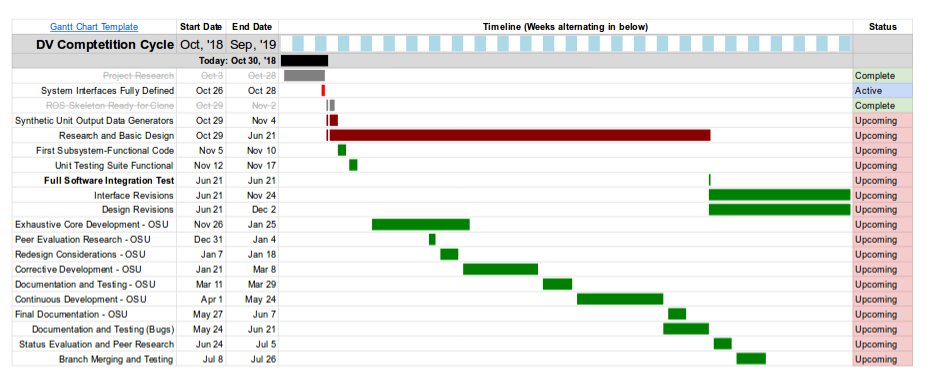
\includegraphics[scale=0.5]{GanttChart_v1.png}
\end{center}

\end{document}
